\section{Pre processing}
\label{sec:pre-proc}

\scolli{Usa questa macro per scrivere commenti}

I dati analizzati sono stati forniti in formato Excel dall'ufficio xxx\scolli{che ufficio?}
presentando quindi una struttura tabellare composta da una serie di campi.

Per consetire un'analisi efficace e priva di errori è stato necessario effettuare una fase di
preprocessing volto a corregge e migliorare la qualità e coerenza dei dati e a scomporre il dataset.

I file forniti presentano al loro interno:
\begin{itemize}
    \item Docenti e ricercatori.
    \item Coperture degli insegnamenti dei vari corsi di laurea.
\end{itemize}

Dopo un approfondita analisi di questi file abbiamo deciso di considerare rilevanti per l'analisi solo alcuni campi.
Nel file dei docenti abbiamo considerato rilevanti solo le colonne contententi la matricola, la fascia e
il settore scientifico disciplinare (SSD).
Nel file relativo alle coperture abbiamo considerato rilevanti solo le colonne contenenti
la matricola del docente, il codice del tipo di corso, il codice del corso di laurea, il settore scientifico disciplinare (SSD).

Per riuscire ad ottenere i dati sopra descritti ben definiti abbiamo effettuato una serie di operazioni di preprocessing per migliorare la qualità dei
dati, così da facilitare l'automatizzazione del workflow generale.

La maggior parte delle operazioni sono state svolte sul file contentente le coperture degli insegnamenti, e sono raggruppabili nei seguenti macroprocessi:
\begin{itemize}
    \item Gestione delle righe contententi una o più colonne vuote.
    \item Scomposizione dei dataset, suddivisione dei dati in sottoinsiemi più piccoli e gestibili.
    \item Identificazione dei casi particolari in modo univoco ed automatizzato.
\end{itemize}

Le righe completamente vuote sono state rimosse in quanto non rilevanti per l'analisi, e le righe che presentano le colonne relative al docente (matricola, nome e cognome) vuote sono state
isolate all'interno di un file separato in quanto rappresentano degli insegnamenti non assegnati ad alcun docente (`insegnamenti_senza_docente.xlsx`).

A questo punto abbiamo suddiviso i dati in sottoinsiemi più piccoli e gestibili.
Come prima cosa abbiamo suddiviso le righe che presentano gli insegnamenti tenuti dai docenti/ricercatori e gli insegnamenti tenuti dai docenti a contratto.

Per fare ciò abbiamo sfruttato il file dei docenti che ci è stato fornito, utilizzato la colonna contentente la matricola per identificare ed estrarre, in due file separati,
le righe relative ai docenti a contratto (`docenti_a_contratto.xlsx') e quelle relative ai docenti a tempo indeterminato (`coperture.xlsx').

In fine dopo aver suddiviso i dati in questo modo abbiamo proceduto con l'identificazione dei casi particolari,
cercando di identificare questi casi tramite un controllo combinato tra due colonne.
I casi particolari che abbiamo identificato sono quelli per i corsi di laurea specifici riportati nella seguente tabella:
\begin{figure}[h]
    \centering
    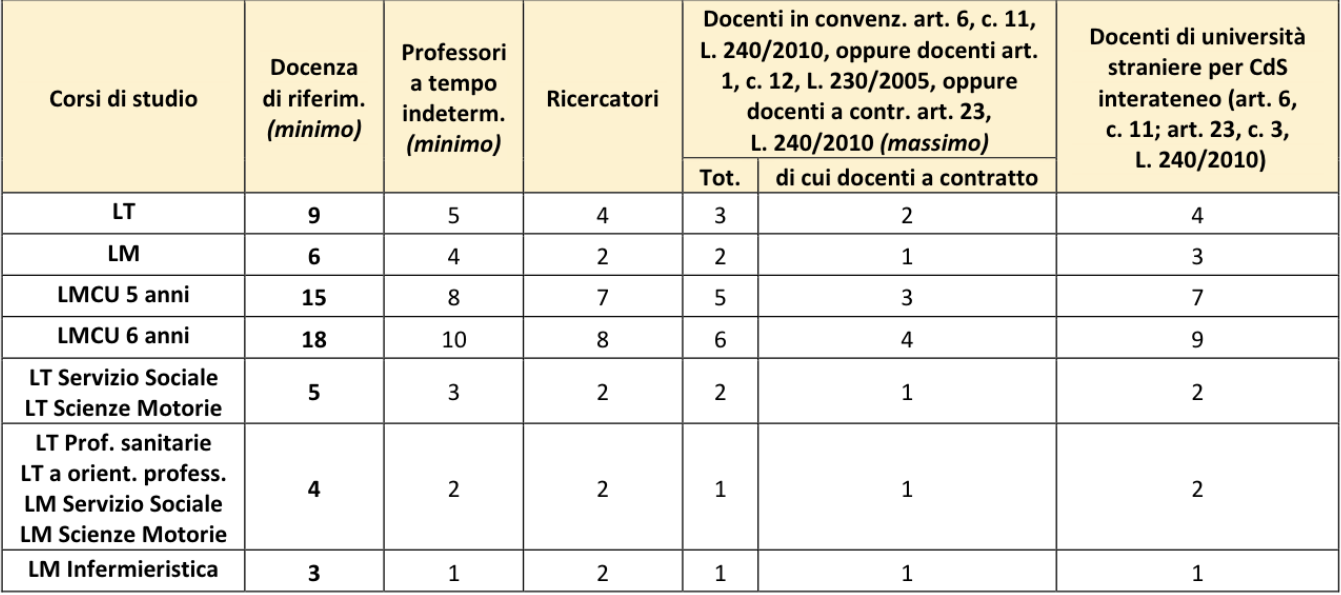
\includegraphics[width=0.8\textwidth]{images/tabella_ministeriale.png}
    \caption{Casi particolari}
    \label{fig:casi_particolari}
\end{figure}
Per fare ciò abbiamo seguito la seguente logica per ogni caso adattandola al corso da verificare.
Prendendo come esempio la laurea triennale di Servizio Sociale abbiamo sostituito il codice del tipo del corso (precedente L)



\subsection{Gestione dei casi particolari}

\subsection{Scomposizione dei dataset}
% \subsection{Dati dei docenti}

% \subsection{Dati delle coperture}




When submitting manuscripts using \LaTeX, a PDF file must also be included. 
Articles should be between 6,000 and 10,000 words, encompassing all text, tables, and figures. 
A concise and descriptive title must be included, and it is essential to list all contributing authors in the submission, along with their email addresses, names, and affiliations.

\subsection{Subsection 1}

Ensure headings are concise and clearly indicate the hierarchy. 
Use sparingly and identify with consecutive numbers in square brackets.
Submit figures (such as \cref{fig-1} electronically at the highest resolution. Number figures consecutively with clear captions.


% \begin{figure}[ht]
%  \centering
%  \makebox[\textwidth][c]{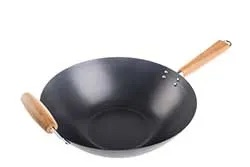
\includegraphics[width=1\textwidth]{images/padella.jpeg}}%
%  \caption{Una padella}
%  \label{fig-1}
% \end{figure}

\subsection{Subsection 2}
\textbf{Emerald Publishing} accepts formats such as .ai, .eps, .jpeg, .bmp, and .tif. Electronic figures created in other applications should be provided in their original formats. 
Additionally, these figures should either be copied and pasted into a blank MS Word document or submitted as a PDF file.